%%%%%%%%%%%%%%%%%%%%%%%%%%%%%%%%%%%%%%%%%%%%%%%%%%%%%%%%%%%
% Organización del proyecto
\section{Organización del proyecto}\label{organizacion:organizacion-del-proyecto}

Dado que el proyecto será manejado por personas en distintos sistemas operativos es vital mantener una coherencia en el orden y la estructura de los archivos y directorios del proyecto.

A continuación, se presenta una propuesta base que considera tanto los ficheros del código como los del diseño artístico:

\subsection{Árbol de directorios}\label{organizacion:arbol-de-directorios}

\begin{itemize}
\item \textbf{Design:} Esta carpeta contiene todos los archivos del diseño de arte del juego (música, sonidos, sprites, tilesets, bocetos, dibujos, animación, etc.). Es de uso para artistas y desarrolladores y su organización muy probablemente se irá modificando en el tiempo. \emph{Ningún archivo dentro de esta carpeta debe ser referenciado por el código}, por lo mismo permite mayor libertad para ajustar nombres y ubicaciones. Más información al respecto en el apartado \nameref{organizacion:nombres-de-archivos}.

\item \textbf{addons:} Carpeta creada por \lsc{GUT} (unittest) y otros plugins de Godot.

\item \textbf{docs:} Contiene toda la documentación de librerías, licencias, \lsc{API}, \lsc{SDK}, manuales, ToDo, apuntes, notas de compilación y configuración relevante para el desarrollo del software.

\item \textbf{export:} Contiene binarios para distintas plataformas del juego y librerías necesarias para su compilación (Por ejemplo librerías propietarias para generar los binarios de una consola).

\item \textbf{locales:} Contiene todos los ficheros relativos a la i18n. Es la carpeta que utilizarán los traductores y desde donde el juego debe tomar todos los strings y los assets correspondientes (assets con texto).

\item \textbf{src:} Probablemente la carpeta principal para el desarrollo técnico. Además del código fuente del programa contendrá todo lo relativo a nodos, escenas, assets, librerías y scripts. La estructura de esta carpeta será utilizada por el proyecto dentro de Godot.

Una consideración importante para mantener la organización de los archivos de una forma que sea coherente con la abstracción de \textit{escenas y nodos}, es crear cada escena dentro de su propia carpeta. Aquí, además del archivo \lsc{TSCN}, deberían estar todos los assets que utiliza la escena para evitar cualquier problemas de dependencias. La idea es poder mover o copiar la carpeta de ubicación y que todo siga funcionando.

\begin{lstlisting}
$ ls src/characters/player/tyanka/
animations/
    tyanka_walk_01.png
    tyanka_walk_02.png
    tyanka_jump_01.png
    etc.
portraits/
    tyanka_portrait_angry_01.png
    tyanka_portrait_angry_02.png
    tyanka_portrait_happy_01.png
    etc.
powers/
    animal_spirit.gd
    palin_shield.gd
    palin_whirl.gd
    etc.
tyanka.gd
tyanka.tsc
tyanka_stats.json
\end{lstlisting}

Si muchas escenas están utilizando los mismos sprites, probablemente se trate de archivos que deberían procesarse e ir dentro de la carpeta \textbf{shared} (detallada más adelante).

A continuación la organización preliminar de la carpeta \textbf{src}:

\begin{itemize}
	\item \textbf{characters:} Contiene las subcarpetas \lsc{FSM}, enemies, npc y player.

	\item \textbf{game:} Todo lo relativo a los Managers, lógica y mecánicas del juego.

	\item \textbf{items:} Todo lo relativo a ítems. A priori dividir en armors, utility y weapons.

	\item \textbf{levels:} Escenas de niveles organizadas en distintas subcarpetas. Contemplar una ubicación para diversos templates.

	\item \textbf{ui:} Todo lo relativo a las escenas de la interfaz gráfica.
\end{itemize}

\item \textbf{shared:} Colección de todos los assets y resources compartidos por más de una escena. Por ejemplo: fuentes tipográficas, música, tilesets, sprites, assets genéricos, etc.
\end{itemize}

\subsubsection*{Diagrama del árbol de directorios.}
\begin{figure}[H]
\centering
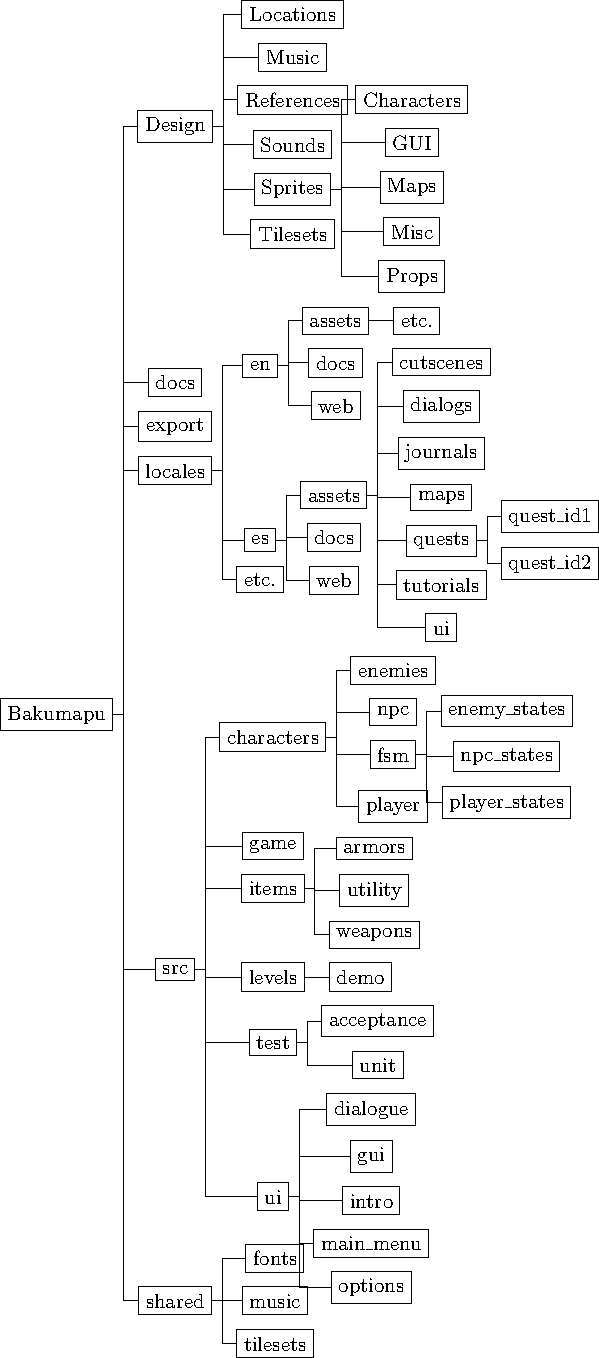
\includegraphics[height=0.93\textheight]{imágenes/arbol_proyecto}
\label{fig:arbolproyecto}
\end{figure}

\subsection{Nombres de archivos}\label{organizacion:nombres-de-archivos}

En términos generales estas son las consideraciones importantes:

\begin{enumerate}
  \item Los nombres solo podrán contener letras \textbf{a-z}, números \textbf{0-9} y guión medio “\textbf{-}” y bajo “\textbf{_}”. No deberán contener acentos, ni eñe, ni espacios.
  
  \item Todos los nombres de archivos deben estar en inglés.
  
  \item Por compatibilidad con sistemas Windows, todos los nombres deben estar en minúscula y seguir el estilo \href{https://en.wikipedia.org/wiki/Snake_case}{snake_case} (palabras en minúscula separadas por guiones bajos “_”). Tener mucho ojo con esto porque un error puede enredar bastante el asunto en \lsc{GIT}.
\end{enumerate}

La carpeta Design tendrá mayor libertad en los nombres ya que los archivos no serán referenciados por el código; no obstante se sugiere seguir los mismos principios.

\subsection{Nombres de ramas y tarjetas}\label{organizacion:nombres-de-ramas}
Ya que las ramas del repositorio \lsc{GIT} y las tarjetas del tablero Kanban tienen su origen en la misma tarea designada por el equipo de desarrollo, para mantener un seguimiento más riguroso y tener mejor información compartirán un mismo nombre. Este nombre será designado al momento de establecer la tarea y deberá cumplir las especificaciones detalladas a continuación.

% Hacer tabla resumen con códigos de nombres.
\todoii{ToDo: Tabla resumen de archivos}{Hacer tabla resumen con códigos de nombres}

Los siguientes nombres corresponden a cada subrama:
\begin{enumerate}
\item Rama de features: \lsc{ft-}
\item Rama de bugs: \lsc{bug-}
\item Rama de patches: \lsc{patch-}
Los patches son cambios al código motivados por features nuevas más que por problemas.
\end{enumerate}

Así, tareas relacionadas con algún elemento de la interfaz gráfica del juego tendrán el nombre de “ui-”

Las ramas con nombres con los que se va a interactuar son las de features y bugs.
Las ramas de nombre fijo
Hay tres tipos de subramas, ramas de features, ramas de bugs y ramas de patch
